\begin{priprava}{7}{}{Urejenost racionalnih števil}{Racionalna števila}{frontalna}{drsnice, projekcija, tabla}

    \section{Urejenost racionalnih števil}

            
    
    Za ulomka $\dfrac{x}{y}$ in $\dfrac{z}{w}$ ($y,w\notin\{0\}$) velja natanko ena izmed treh možnosti:
    
    \begin{enumerate}
        \item prvi ulomek je večji od drugega $\dfrac{x}{y}\geq\dfrac{z}{w}$ natanko tedaj, ko je $xw\geq yz$;
        \item drugi ulomek je večji od prvega $\dfrac{x}{y}\leq\dfrac{z}{w}$ natanko tedaj, ko je $xw\leq yz$;
        \item ulomka sta enaka $\dfrac{x}{y}=\dfrac{z}{w}$ natanko tedaj, ko je $xw=yz$ oziroma $\dfrac{x}{y}\leq\dfrac{z}{w} \land \dfrac{x}{y}\geq\dfrac{z}{w}$.
    \end{enumerate}


    Enaka ulomka predstavljata isto racionalno število.

    ~

    Slika večjega racionalnega števila \textcolor{red}{$\dfrac{x}{y}$} je na številski premici desno od slike manjšega racionalnega števila \textcolor{green}{$\dfrac{z}{w}$}.
\begin{figure}[H]
    \centering
    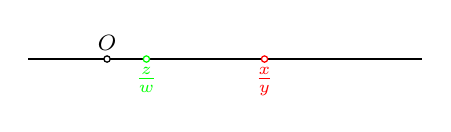
\begin{tikzpicture}
        % \clip (0,0) rectangle (14.000000,10.000000);
        {\footnotesize
        
        % Drawing segment A B
        \draw [line width=0.016cm] (1.000000,1.500000) -- (1.960000,1.500000);%
        \draw [line width=0.016cm] (2.040000,1.500000) -- (2.460000,1.500000);%
        \draw [line width=0.016cm] (2.540000,1.500000) -- (3.960000,1.500000);%
        \draw [line width=0.016cm] (4.040000,1.500000) -- (6.000000,1.500000);%
        
        % Marking point O by circle
        \draw [line width=0.016cm] (2.000000,1.500000) circle (0.040000);%
        \draw (2.000000,1.500000) node [anchor=south] { $O$ };%
        
        % Changing color 255 0 0
        \definecolor{r255g0b0}{rgb}{1.000000,0.000000,0.000000}%
        \color{r255g0b0}% 
        
        % Marking point \frac{x}{y} by circle
        \draw [line width=0.016cm] (4.000000,1.500000) circle (0.040000);%
        \draw (4.000000,1.500000) node [anchor=north] { $\frac{x}{y}$ };%
        
        % Changing color 0 255 0
        \definecolor{r0g255b0}{rgb}{0.000000,1.000000,0.000000}%
        \color{r0g255b0}% 
        
        % Marking point \frac{z}{w} by circle
        \draw [line width=0.016cm] (2.500000,1.500000) circle (0.040000);%
        \draw (2.500000,1.500000) node [anchor=north] { $\frac{z}{w}$ };%
        \color{black}
        }
    \end{tikzpicture}
\end{figure}    


Slike pozitivnih racionalnih števil ležijo desno, slike negativnih racionalnih števil pa levo od koordinatnega izhodišča.
    \begin{figure}[H]
        \centering
        \begin{tikzpicture}
            
            % \clip (0,0) rectangle (14.000000,10.000000);
            {\footnotesize
            
            % Drawing segment A B
            \draw [line width=0.016cm] (1.000000,1.500000) -- (3.460000,1.500000);%
            \draw [line width=0.016cm] (3.540000,1.500000) -- (6.000000,1.500000);%
            
            % Changing color 255 0 0
            \definecolor{r255g0b0}{rgb}{1.000000,0.000000,0.000000}%
            \color{r255g0b0}% 
            
            % Drawing segment B O
            \draw [line width=0.016cm] (6.000000,1.500000) -- (3.540000,1.500000);%
            
            % Marking point pozitivna_tevila
            \draw (4.750000,1.500000) node [anchor=north] { $pozitivna~ števila$ };%
            \draw (4.750000,1.500000) node [anchor=south] { $\mathbb{Q}^+$ };%
            
            % Changing color 0 255 0
            \definecolor{r0g255b0}{rgb}{0.000000,1.000000,0.000000}%
            \color{r0g255b0}% 
            
            % Drawing segment O A
            \draw [line width=0.016cm] (3.460000,1.500000) -- (1.000000,1.500000);%
            
            % Marking point negativna_tevila
            \draw (2.250000,1.500000) node [anchor=north] { $negativna~ števila$ };%
            \draw (2.250000,1.500000) node [anchor=south] { $\mathbb{Q}^-$ };%
            
            % Changing color 0 0 0
            \definecolor{r0g0b0}{rgb}{0.000000,0.000000,0.000000}%
            \color{r0g0b0}% 
            
            % Marking point O by circle
            \draw [line width=0.032cm] (3.500000,1.500000) circle (0.040000);%
            \draw (3.500000,1.500000) node [anchor=south] { $O$ };%
            \color{black}
            }
        \end{tikzpicture}
    \end{figure}

    

    V množici ulomkov velja, da je vsak negativen ulomek manjši od vsakega pozitivnega ulomka.


    ~

    Množica racionalnih števil je \textbf{linearno urejena} z relacijo \textit{biti manjši ali enak} ($\leq$) oziroma \textit{biti večji ali enak} ($\geq$). 
    
    Za to relacijo linearne urejenosti veljajo naslednje lastnosti:

    \begin{itemize}
        \item \textbf{refleksivnost}: $\forall \dfrac{x}{y}\in\mathbb{Q}: \dfrac{x}{y}\leq\dfrac{x}{y}$;
        \item \textbf{antisimetričnost}: $\forall \dfrac{x}{y},\dfrac{z}{w}\in\mathbb{Q}: \dfrac{x}{y}\leq\dfrac{z}{w}  \land \dfrac{z}{w}\leq\dfrac{x}{y} \Rightarrow \dfrac{x}{y}=\dfrac{z}{w}$;
        \item \textbf{tranzitivnost}: $\forall \dfrac{x}{y},\dfrac{z}{w},\dfrac{r}{q}\in\mathbb{Q}: \dfrac{x}{y}\leq\dfrac{z}{w}  \land \dfrac{z}{w}\leq\dfrac{r}{q} \Rightarrow \dfrac{x}{y}\leq\dfrac{r}{q}$ in 
        \item \textbf{stroga sovisnost}: $\forall \dfrac{x}{y},\dfrac{z}{w}\in\mathbb{Q}: \dfrac{x}{y}\leq\dfrac{z}{w}  \lor \dfrac{z}{w}\leq\dfrac{x}{y}$.
    \end{itemize}

~

    Množica racionalnih števil pa je tudi \textbf{delno urejena}, in sicer z relacijo \textit{biti manjši} ($<$) oziroma \textit{biti večji} ($>$). 

    Tedaj veljajo le lastnosti: \textbf{refleksivnost}, \textbf{antisimetričnost} in \textbf{tranzitivnost}.


    ~

    Pri množenju neenakosti s pozitivnim številom se znak neenakosti ohrani.
    $$ \dfrac{x}{y}<\dfrac{z}{w} \quad \wedge \quad \dfrac{r}{q}>0 \quad \Rightarrow \quad \dfrac{x}{y}\cdot\dfrac{r}{q}<\dfrac{z}{w}\cdot\dfrac{r}{q} $$

    

    Pri množenju neenakosti s negativnim številom se znak neenakosti obrne.
    $$ \dfrac{x}{y}<\dfrac{z}{w} \quad \wedge \quad \dfrac{r}{q}<0 \quad \Rightarrow \quad \dfrac{x}{y}\cdot\dfrac{r}{q}>\dfrac{z}{w}\cdot\dfrac{r}{q} $$


    \subsubsection*{Monotonost vsote}
    Če na obeh straneh neenakosti prištejemo isto število, se neenakost ohrani.
    $$ \dfrac{x}{y}<\dfrac{z}{w} \quad \Rightarrow \quad \dfrac{x}{y}+\dfrac{r}{q}<\dfrac{z}{w}+\dfrac{r}{q} $$


    %%% naloge
    ~
    \begin{naloga}
        Kateri od ulomkov je večji?
        \begin{itemize}
            \item $\frac{3}{7}$, $\frac{3}{8}$ 
            \item $\frac{7}{3}$, $\frac{8}{3}$ 
            \item $\frac{2}{5}$, $\frac{3}{10}$ 
            \item $\frac{1}{100}$, $\frac{1}{200}$ 
        \end{itemize}
    \end{naloga}

    \begin{naloga}
        Katero število je za $\frac{3}{5}$ večje od $\frac{2}{3}$?
        
    \end{naloga}

    \begin{naloga}
        Katero število je za $\frac{1}{3}$ manjše od $\frac{7}{9}$?
        
    \end{naloga}

    \begin{naloga}
        Ulomke uredite po velikosti od večjega k manjšemu.
        \begin{itemize}
            \item $\frac{2}{5}$, $\frac{3}{10}$, $\frac{8}{9}$ in $\frac{7}{8}$ 
            \item $-\frac{1}{2}$, $\frac{-1}{3}$, $\frac{-3}{4}$ in $\frac{2}{-5}$ 
        \end{itemize}
    \end{naloga}


    \begin{naloga}
        Ali obstajajo ulomki z imenovalcem $25$, ki so med $\frac{4}{9}$ in $\frac{5}{9}$? Če obstajajo, jih zapišite.
        
    \end{naloga}

    \begin{naloga}
        Ali obstajajo ulomki z imenovalcem $100$, ki so med $\frac{13}{53}$ in $\frac{14}{53}$? Če obstajajo, jih zapišite.
        
    \end{naloga}



\end{priprava}